\documentclass{book}
\usepackage[a4paper,top=2.5cm,bottom=2.5cm,left=2.5cm,right=2.5cm]{geometry}
\usepackage{makeidx}
\usepackage{natbib}
\usepackage{graphicx}
\usepackage{multicol}
\usepackage{float}
\usepackage{listings}
\usepackage{color}
\usepackage{ifthen}
\usepackage[table]{xcolor}
\usepackage{textcomp}
\usepackage{alltt}
\usepackage{ifpdf}
\ifpdf
\usepackage[pdftex,
            pagebackref=true,
            colorlinks=true,
            linkcolor=blue,
            unicode
           ]{hyperref}
\else
\usepackage[ps2pdf,
            pagebackref=true,
            colorlinks=true,
            linkcolor=blue,
            unicode
           ]{hyperref}
\usepackage{pspicture}
\fi
\usepackage[utf8]{inputenc}
\usepackage{polski}
\usepackage[T1]{fontenc}

\usepackage{mathptmx}
\usepackage[scaled=.90]{helvet}
\usepackage{courier}
\usepackage{sectsty}
\usepackage{amssymb}
\usepackage[titles]{tocloft}
\usepackage{doxygen}
\lstset{language=C++,inputencoding=utf8,basicstyle=\footnotesize,breaklines=true,breakatwhitespace=true,tabsize=4,numbers=left }
\makeindex
\setcounter{tocdepth}{3}
\renewcommand{\footrulewidth}{0.4pt}
\renewcommand{\familydefault}{\sfdefault}
\hfuzz=15pt
\setlength{\emergencystretch}{15pt}
\hbadness=750
\tolerance=750
\begin{document}
\hypersetup{pageanchor=false,citecolor=blue}
\begin{titlepage}
\vspace*{7cm}
\begin{center}
{\Large Tablica asocjacyjna \\[1ex]\large 0.\-1 }\\
\vspace*{1cm}
{\large Wygenerowano przez Doxygen 1.8.3.1}\\
\vspace*{0.5cm}
{\small N, 6 kwi 2014 12:20:34}\\
\end{center}
\end{titlepage}
\clearemptydoublepage
\pagenumbering{roman}
\tableofcontents
\clearemptydoublepage
\pagenumbering{arabic}
\hypersetup{pageanchor=true,citecolor=blue}
\chapter{Dokumentacja zadania lab6}
\label{index}\hypertarget{index}{}\begin{DoxyAuthor}{Autor}
Karolina Morawska 
\end{DoxyAuthor}
\begin{DoxyDate}{Data}
16.\-03.\-2014 
\end{DoxyDate}
\begin{DoxyVersion}{Wersja}
0.\-2 
\end{DoxyVersion}

\chapter{Indeks klas}
\section{Lista klas}
Tutaj znajdują się klasy, struktury, unie i interfejsy wraz z ich krótkimi opisami\-:\begin{DoxyCompactList}
\item\contentsline{section}{\hyperlink{class_n_o_d_e}{N\-O\-D\-E} \\*Modeluje pojęcie \hyperlink{class_n_o_d_e}{N\-O\-D\-E} ,czyli wezel. Klasa modeluje pojęcie node . Jej atrybutem są pola zawierające wskaźnik na lewy ,prawy węzeł i wartość }{\pageref{class_n_o_d_e}}{}
\item\contentsline{section}{\hyperlink{class_para}{Para} \\*Modeluje pojęcie \hyperlink{class_para}{Para}. Klasa modeluje pojęcie para . Jej atrybutem są pola zawierające klucz i wartość }{\pageref{class_para}}{}
\item\contentsline{section}{\hyperlink{classper}{per$<$ K, W $>$} \\*Modeluje pojęcie per. Klasa modeluje pojęcie per(para) . Jej atrybutem są pola zawierające klucz i wartość }{\pageref{classper}}{}
\item\contentsline{section}{\hyperlink{class_tablicaas}{Tablicaas$<$ K, W $>$} \\*Modeluje pojęcie \hyperlink{class_tablicaas}{Tablicaas}. Klasa modeluje pojęcie Tablica asocjacyjna . Jej atrybutem są pola zawierające klucz i wartość }{\pageref{class_tablicaas}}{}
\item\contentsline{section}{\hyperlink{class_tree}{Tree} \\*Modeluje pojęcie \hyperlink{class_para}{Para}. Klasa modeluje pojęcie para . Jej atrybutem jest pole zawierajace root(korzen) }{\pageref{class_tree}}{}
\end{DoxyCompactList}

\chapter{Indeks plików}
\section{Lista plików}
Tutaj znajduje się lista wszystkich plików z ich krótkimi opisami\-:\begin{DoxyCompactList}
\item\contentsline{section}{\hyperlink{czas_8hh}{czas.\-hh} }{\pageref{czas_8hh}}{}
\item\contentsline{section}{\hyperlink{dzialania_8cpp}{dzialania.\-cpp} }{\pageref{dzialania_8cpp}}{}
\item\contentsline{section}{\hyperlink{dzialania_8hh}{dzialania.\-hh} }{\pageref{dzialania_8hh}}{}
\item\contentsline{section}{\hyperlink{kolejka_8hh}{kolejka.\-hh} }{\pageref{kolejka_8hh}}{}
\item\contentsline{section}{\hyperlink{main_8cpp}{main.\-cpp} }{\pageref{main_8cpp}}{}
\item\contentsline{section}{\hyperlink{stos_8hh}{stos.\-hh} }{\pageref{stos_8hh}}{}
\item\contentsline{section}{\hyperlink{stos2_8hh}{stos2.\-hh} }{\pageref{stos2_8hh}}{}
\item\contentsline{section}{\hyperlink{stoslista_8hh}{stoslista.\-hh} }{\pageref{stoslista_8hh}}{}
\item\contentsline{section}{\hyperlink{tablica_8cpp}{tablica.\-cpp} }{\pageref{tablica_8cpp}}{}
\item\contentsline{section}{\hyperlink{tablica_8hh}{tablica.\-hh} }{\pageref{tablica_8hh}}{}
\end{DoxyCompactList}

\chapter{Dokumentacja klas}
\hypertarget{classper}{\section{Dokumentacja szablonu klasy per$<$ K, W $>$}
\label{classper}\index{per$<$ K, W $>$@{per$<$ K, W $>$}}
}


Modeluje pojęcie per. Klasa modeluje pojęcie per(para) . Jej atrybutem są pola zawierające klucz i wartość.  




{\ttfamily \#include $<$per.\-hh$>$}

\subsection*{Metody publiczne}
\begin{DoxyCompactItemize}
\item 
\hyperlink{classper_a73013b168f465e358ce0371a730a0bfa}{per} (K \-\_\-key, W \-\_\-wartosc)
\item 
\hyperlink{classper_a15a9c5b538d2c25c8b2492f0acfbba89}{per} ()
\end{DoxyCompactItemize}
\subsection*{Atrybuty publiczne}
\begin{DoxyCompactItemize}
\item 
K \hyperlink{classper_a33ecddc68cd15fc35c4f7487b4f2705d}{key}
\begin{DoxyCompactList}\small\item\em Inicjalizuje wartosc klucz. \end{DoxyCompactList}\item 
W $\ast$ \hyperlink{classper_a226a74072ab3ff12f6c31e27190762a0}{wartosc}
\begin{DoxyCompactList}\small\item\em Inicjalizuje wartosc zmiennej wartość. \end{DoxyCompactList}\end{DoxyCompactItemize}


\subsection{Opis szczegółowy}
\subsubsection*{template$<$typename K, typename W$>$class per$<$ K, W $>$}



Definicja w linii 31 pliku per.\-hh.



\subsection{Dokumentacja konstruktora i destruktora}
\hypertarget{classper_a73013b168f465e358ce0371a730a0bfa}{\index{per@{per}!per@{per}}
\index{per@{per}!per@{per}}
\subsubsection[{per}]{\setlength{\rightskip}{0pt plus 5cm}template$<$typename K, typename W$>$ {\bf per}$<$ K, W $>$\-::{\bf per} (
\begin{DoxyParamCaption}
\item[{K}]{\-\_\-key, }
\item[{W}]{\-\_\-wartosc}
\end{DoxyParamCaption}
)\hspace{0.3cm}{\ttfamily [inline]}}}\label{classper_a73013b168f465e358ce0371a730a0bfa}


Definicja w linii 41 pliku per.\-hh.

\hypertarget{classper_a15a9c5b538d2c25c8b2492f0acfbba89}{\index{per@{per}!per@{per}}
\index{per@{per}!per@{per}}
\subsubsection[{per}]{\setlength{\rightskip}{0pt plus 5cm}template$<$typename K, typename W$>$ {\bf per}$<$ K, W $>$\-::{\bf per} (
\begin{DoxyParamCaption}
{}
\end{DoxyParamCaption}
)\hspace{0.3cm}{\ttfamily [inline]}}}\label{classper_a15a9c5b538d2c25c8b2492f0acfbba89}


Definicja w linii 47 pliku per.\-hh.



\subsection{Dokumentacja atrybutów składowych}
\hypertarget{classper_a33ecddc68cd15fc35c4f7487b4f2705d}{\index{per@{per}!key@{key}}
\index{key@{key}!per@{per}}
\subsubsection[{key}]{\setlength{\rightskip}{0pt plus 5cm}template$<$typename K, typename W$>$ K {\bf per}$<$ K, W $>$\-::key}}\label{classper_a33ecddc68cd15fc35c4f7487b4f2705d}


Definicja w linii 36 pliku per.\-hh.

\hypertarget{classper_a226a74072ab3ff12f6c31e27190762a0}{\index{per@{per}!wartosc@{wartosc}}
\index{wartosc@{wartosc}!per@{per}}
\subsubsection[{wartosc}]{\setlength{\rightskip}{0pt plus 5cm}template$<$typename K, typename W$>$ W$\ast$ {\bf per}$<$ K, W $>$\-::wartosc}}\label{classper_a226a74072ab3ff12f6c31e27190762a0}


Definicja w linii 40 pliku per.\-hh.



Dokumentacja dla tej klasy została wygenerowana z pliku\-:\begin{DoxyCompactItemize}
\item 
\hyperlink{per_8hh}{per.\-hh}\end{DoxyCompactItemize}

\hypertarget{class_tablicaas}{\section{Dokumentacja szablonu klasy Tablicaas$<$ K, W $>$}
\label{class_tablicaas}\index{Tablicaas$<$ K, W $>$@{Tablicaas$<$ K, W $>$}}
}


Modeluje pojęcie \hyperlink{class_tablicaas}{Tablicaas}. Klasa modeluje pojęcie Tablica asocjacyjna . Jej atrybutem są pola zawierające klucz i wartość.  




{\ttfamily \#include $<$tablicaas.\-hh$>$}

\subsection*{Metody publiczne}
\begin{DoxyCompactItemize}
\item 
void \hyperlink{class_tablicaas_ac97f4cb96d75a56448b9ed5a44b60826}{dodaj} (\hyperlink{classper}{per}$<$ K, W $>$ para)
\begin{DoxyCompactList}\small\item\em Dodaje parę-\/wartość i klucz. Dodatkowo zmienna ilosc elementow zostaje zwiekszona. \end{DoxyCompactList}\item 
void \hyperlink{class_tablicaas_aa961a5575d84d6f5762063f719879ae1}{usun} (K key)
\begin{DoxyCompactList}\small\item\em Metoda która usuwa klucz. Dodatkowo zmienna ilosc elementow zostaje zmniejszona. \end{DoxyCompactList}\item 
W \hyperlink{class_tablicaas_a329ae3086855ea056a5249430de4b5f3}{pobierz} (K key)
\begin{DoxyCompactList}\small\item\em Pobiera klucz. /return Zwraca zmienna o nazwie wartosc. \end{DoxyCompactList}\item 
bool \hyperlink{class_tablicaas_aff9f43c59bcb48c6f8fee095517960c9}{czypusta} ()
\begin{DoxyCompactList}\small\item\em Sprawdza zawartość tablicy. \end{DoxyCompactList}\item 
int \hyperlink{class_tablicaas_a2a6376d5554f6e028baf1c64f182fedc}{size} ()
\begin{DoxyCompactList}\small\item\em Podaje rozmiar. \end{DoxyCompactList}\item 
W \& \hyperlink{class_tablicaas_aacc5f2336e38656f946e46076794a071}{operator\mbox{[}$\,$\mbox{]}} (K key)
\begin{DoxyCompactList}\small\item\em Przeciążenie operatora indeksującego. \end{DoxyCompactList}\item 
int \hyperlink{class_tablicaas_a40a1e67d84970aaf04581fd6e0346220}{haszstring} (string key) const 
\begin{DoxyCompactList}\small\item\em Funkcja haszująca dla obiektów typu string. \end{DoxyCompactList}\end{DoxyCompactItemize}
\subsection*{Atrybuty publiczne}
\begin{DoxyCompactItemize}
\item 
\hyperlink{classper}{per}$<$ K, W $>$ \hyperlink{class_tablicaas_a5f06a7cdb8f1b32a7791381c7c815d5e}{Tab} \mbox{[}\hyperlink{tablicaas_8hh_aa50aa866c5823769bb02e986d29a0589}{R\-O\-Z\-M\-I\-A\-R}\mbox{]}
\begin{DoxyCompactList}\small\item\em Wykorzystuje pola z klasy per. \end{DoxyCompactList}\end{DoxyCompactItemize}
\subsection*{Statyczne atrybuty publiczne}
\begin{DoxyCompactItemize}
\item 
static int \hyperlink{class_tablicaas_a6710dabb371ab39cb600fa7fcf2e06ed}{zmienna} =0
\begin{DoxyCompactList}\small\item\em Pomocnicza zmienna statyczna. \end{DoxyCompactList}\end{DoxyCompactItemize}


\subsection{Opis szczegółowy}
\subsubsection*{template$<$typename K, typename W$>$class Tablicaas$<$ K, W $>$}



Definicja w linii 28 pliku tablicaas.\-hh.



\subsection{Dokumentacja funkcji składowych}
\hypertarget{class_tablicaas_aff9f43c59bcb48c6f8fee095517960c9}{\index{Tablicaas@{Tablicaas}!czypusta@{czypusta}}
\index{czypusta@{czypusta}!Tablicaas@{Tablicaas}}
\subsubsection[{czypusta}]{\setlength{\rightskip}{0pt plus 5cm}template$<$typename K, typename W$>$ bool {\bf Tablicaas}$<$ K, W $>$\-::czypusta (
\begin{DoxyParamCaption}
{}
\end{DoxyParamCaption}
)\hspace{0.3cm}{\ttfamily [inline]}}}\label{class_tablicaas_aff9f43c59bcb48c6f8fee095517960c9}
\begin{DoxyReturn}{Zwraca}
Metoda porownuje zmienna i zwraca true jeśli zmienna jest równa 0 i false w przeciwnym wypadku. 
\end{DoxyReturn}


Definicja w linii 55 pliku tablicaas.\-hh.



Oto graf wywoływań tej funkcji\-:
\nopagebreak
\begin{figure}[H]
\begin{center}
\leavevmode
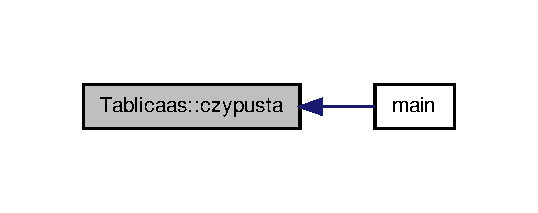
\includegraphics[width=258pt]{class_tablicaas_aff9f43c59bcb48c6f8fee095517960c9_icgraph}
\end{center}
\end{figure}


\hypertarget{class_tablicaas_ac97f4cb96d75a56448b9ed5a44b60826}{\index{Tablicaas@{Tablicaas}!dodaj@{dodaj}}
\index{dodaj@{dodaj}!Tablicaas@{Tablicaas}}
\subsubsection[{dodaj}]{\setlength{\rightskip}{0pt plus 5cm}template$<$typename K , typename W $>$ void {\bf Tablicaas}$<$ K, W $>$\-::dodaj (
\begin{DoxyParamCaption}
\item[{{\bf per}$<$ K, W $>$}]{para}
\end{DoxyParamCaption}
)}}\label{class_tablicaas_ac97f4cb96d75a56448b9ed5a44b60826}


Definicja w linii 85 pliku tablicaas.\-hh.



Oto graf wywoływań tej funkcji\-:
\nopagebreak
\begin{figure}[H]
\begin{center}
\leavevmode
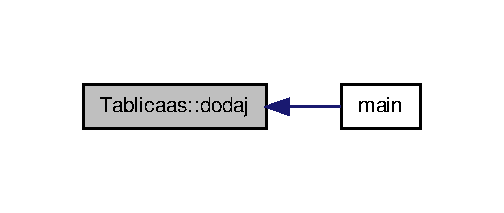
\includegraphics[width=242pt]{class_tablicaas_ac97f4cb96d75a56448b9ed5a44b60826_icgraph}
\end{center}
\end{figure}


\hypertarget{class_tablicaas_a40a1e67d84970aaf04581fd6e0346220}{\index{Tablicaas@{Tablicaas}!haszstring@{haszstring}}
\index{haszstring@{haszstring}!Tablicaas@{Tablicaas}}
\subsubsection[{haszstring}]{\setlength{\rightskip}{0pt plus 5cm}template$<$typename K, typename W$>$ int {\bf Tablicaas}$<$ K, W $>$\-::haszstring (
\begin{DoxyParamCaption}
\item[{string}]{key}
\end{DoxyParamCaption}
) const\hspace{0.3cm}{\ttfamily [inline]}}}\label{class_tablicaas_a40a1e67d84970aaf04581fd6e0346220}


Definicja w linii 77 pliku tablicaas.\-hh.

\hypertarget{class_tablicaas_aacc5f2336e38656f946e46076794a071}{\index{Tablicaas@{Tablicaas}!operator\mbox{[}$\,$\mbox{]}@{operator[]}}
\index{operator\mbox{[}$\,$\mbox{]}@{operator[]}!Tablicaas@{Tablicaas}}
\subsubsection[{operator[]}]{\setlength{\rightskip}{0pt plus 5cm}template$<$typename K , typename W $>$ W \& {\bf Tablicaas}$<$ K, W $>$\-::operator\mbox{[}$\,$\mbox{]} (
\begin{DoxyParamCaption}
\item[{K}]{key}
\end{DoxyParamCaption}
)}}\label{class_tablicaas_aacc5f2336e38656f946e46076794a071}
\begin{DoxyReturn}{Zwraca}
Zwraca wartosc. 
\end{DoxyReturn}


Definicja w linii 105 pliku tablicaas.\-hh.

\hypertarget{class_tablicaas_a329ae3086855ea056a5249430de4b5f3}{\index{Tablicaas@{Tablicaas}!pobierz@{pobierz}}
\index{pobierz@{pobierz}!Tablicaas@{Tablicaas}}
\subsubsection[{pobierz}]{\setlength{\rightskip}{0pt plus 5cm}template$<$typename K , typename W $>$ W {\bf Tablicaas}$<$ K, W $>$\-::pobierz (
\begin{DoxyParamCaption}
\item[{K}]{key}
\end{DoxyParamCaption}
)}}\label{class_tablicaas_a329ae3086855ea056a5249430de4b5f3}


Definicja w linii 98 pliku tablicaas.\-hh.



Oto graf wywoływań tej funkcji\-:
\nopagebreak
\begin{figure}[H]
\begin{center}
\leavevmode
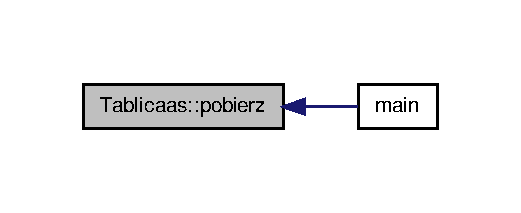
\includegraphics[width=250pt]{class_tablicaas_a329ae3086855ea056a5249430de4b5f3_icgraph}
\end{center}
\end{figure}


\hypertarget{class_tablicaas_a2a6376d5554f6e028baf1c64f182fedc}{\index{Tablicaas@{Tablicaas}!size@{size}}
\index{size@{size}!Tablicaas@{Tablicaas}}
\subsubsection[{size}]{\setlength{\rightskip}{0pt plus 5cm}template$<$typename K, typename W$>$ int {\bf Tablicaas}$<$ K, W $>$\-::size (
\begin{DoxyParamCaption}
{}
\end{DoxyParamCaption}
)\hspace{0.3cm}{\ttfamily [inline]}}}\label{class_tablicaas_a2a6376d5554f6e028baf1c64f182fedc}
\begin{DoxyReturn}{Zwraca}
Zwraca zmienna statyczna. 
\end{DoxyReturn}


Definicja w linii 62 pliku tablicaas.\-hh.

\hypertarget{class_tablicaas_aa961a5575d84d6f5762063f719879ae1}{\index{Tablicaas@{Tablicaas}!usun@{usun}}
\index{usun@{usun}!Tablicaas@{Tablicaas}}
\subsubsection[{usun}]{\setlength{\rightskip}{0pt plus 5cm}template$<$typename K , typename W $>$ void {\bf Tablicaas}$<$ K, W $>$\-::usun (
\begin{DoxyParamCaption}
\item[{K}]{key}
\end{DoxyParamCaption}
)}}\label{class_tablicaas_aa961a5575d84d6f5762063f719879ae1}


Definicja w linii 91 pliku tablicaas.\-hh.



Oto graf wywoływań tej funkcji\-:
\nopagebreak
\begin{figure}[H]
\begin{center}
\leavevmode
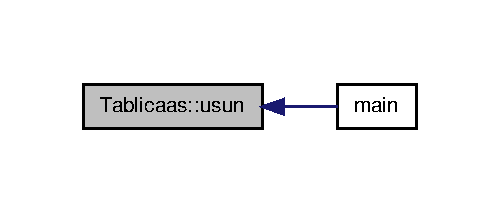
\includegraphics[width=240pt]{class_tablicaas_aa961a5575d84d6f5762063f719879ae1_icgraph}
\end{center}
\end{figure}




\subsection{Dokumentacja atrybutów składowych}
\hypertarget{class_tablicaas_a5f06a7cdb8f1b32a7791381c7c815d5e}{\index{Tablicaas@{Tablicaas}!Tab@{Tab}}
\index{Tab@{Tab}!Tablicaas@{Tablicaas}}
\subsubsection[{Tab}]{\setlength{\rightskip}{0pt plus 5cm}template$<$typename K, typename W$>$ {\bf per}$<$K,W$>$ {\bf Tablicaas}$<$ K, W $>$\-::Tab\mbox{[}{\bf R\-O\-Z\-M\-I\-A\-R}\mbox{]}}}\label{class_tablicaas_a5f06a7cdb8f1b32a7791381c7c815d5e}


Definicja w linii 33 pliku tablicaas.\-hh.

\hypertarget{class_tablicaas_a6710dabb371ab39cb600fa7fcf2e06ed}{\index{Tablicaas@{Tablicaas}!zmienna@{zmienna}}
\index{zmienna@{zmienna}!Tablicaas@{Tablicaas}}
\subsubsection[{zmienna}]{\setlength{\rightskip}{0pt plus 5cm}template$<$typename K, typename W$>$ int {\bf Tablicaas}$<$ K, W $>$\-::zmienna =0\hspace{0.3cm}{\ttfamily [static]}}}\label{class_tablicaas_a6710dabb371ab39cb600fa7fcf2e06ed}


Definicja w linii 68 pliku tablicaas.\-hh.



Dokumentacja dla tej klasy została wygenerowana z plików\-:\begin{DoxyCompactItemize}
\item 
\hyperlink{tablicaas_8hh}{tablicaas.\-hh}\item 
\hyperlink{main_8cpp}{main.\-cpp}\end{DoxyCompactItemize}

\chapter{Dokumentacja plików}
\hypertarget{main_8cpp}{\section{Dokumentacja pliku /home/karolina/\-Pulpit/pamsi/prj/src/main.cpp}
\label{main_8cpp}\index{/home/karolina/\-Pulpit/pamsi/prj/src/main.\-cpp@{/home/karolina/\-Pulpit/pamsi/prj/src/main.\-cpp}}
}
{\ttfamily \#include $<$iostream$>$}\\*
{\ttfamily \#include $<$dzialania.\-hh$>$}\\*
{\ttfamily \#include $<$cstdlib$>$}\\*
Wykres zależności załączania dla main.\-cpp\-:
\subsection*{Funkcje}
\begin{DoxyCompactItemize}
\item 
int \hyperlink{main_8cpp_a3c04138a5bfe5d72780bb7e82a18e627}{main} (int argc, char $\ast$$\ast$argv)
\begin{DoxyCompactList}\small\item\em Funkcja main wykonuje algorytm i sprawdza czas dzialania algorytmu. W funkcji main wykonywane sa operacje \-: -\/\-Wczytywanie pliku z danymi wejsciowym -\/\-Dane sa mnozone razy 2 (w tej chwili wlaczany jest stoper) -\/\-Wczytywanie pliku z danymi sprawdzajacymi -\/\-Sprawdzanie zgodnosci -\/\-Stoper zostaje wylaczony i na wyjsciu programu podany zostaje czas dzialania algorytmu. \end{DoxyCompactList}\end{DoxyCompactItemize}


\subsection{Dokumentacja funkcji}
\hypertarget{main_8cpp_a3c04138a5bfe5d72780bb7e82a18e627}{\index{main.\-cpp@{main.\-cpp}!main@{main}}
\index{main@{main}!main.cpp@{main.\-cpp}}
\subsubsection[{main}]{\setlength{\rightskip}{0pt plus 5cm}int main (
\begin{DoxyParamCaption}
\item[{int}]{argc, }
\item[{char $\ast$$\ast$}]{argv}
\end{DoxyParamCaption}
)}}\label{main_8cpp_a3c04138a5bfe5d72780bb7e82a18e627}


Funkcja main wykonuje algorytm i sprawdza czas dzialania algorytmu. W funkcji main wykonywane sa operacje \-: -\/\-Wczytywanie pliku z danymi wejsciowym -\/\-Dane sa mnozone razy 2 (w tej chwili wlaczany jest stoper) -\/\-Wczytywanie pliku z danymi sprawdzajacymi -\/\-Sprawdzanie zgodnosci -\/\-Stoper zostaje wylaczony i na wyjsciu programu podany zostaje czas dzialania algorytmu. 



Definicja w linii 22 pliku main.\-cpp.


\hypertarget{per_8hh}{\section{Dokumentacja pliku per.\-hh}
\label{per_8hh}\index{per.\-hh@{per.\-hh}}
}


Definicja szablonu klasy Per.  


{\ttfamily \#include $<$string$>$}\\*
{\ttfamily \#include $<$iostream$>$}\\*
Wykres zależności załączania dla per.\-hh\-:\nopagebreak
\begin{figure}[H]
\begin{center}
\leavevmode
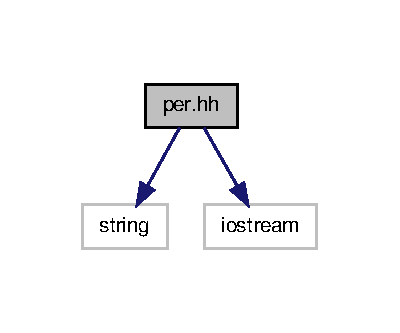
\includegraphics[width=192pt]{per_8hh__incl}
\end{center}
\end{figure}
Ten wykres pokazuje, które pliki bezpośrednio lub pośrednio załączają ten plik\-:\nopagebreak
\begin{figure}[H]
\begin{center}
\leavevmode
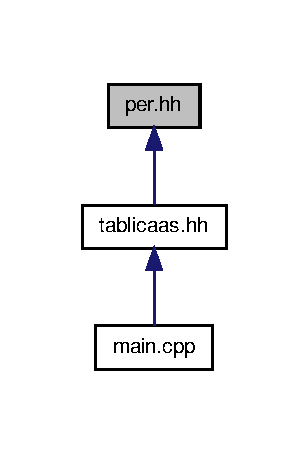
\includegraphics[width=148pt]{per_8hh__dep__incl}
\end{center}
\end{figure}
\subsection*{Komponenty}
\begin{DoxyCompactItemize}
\item 
class \hyperlink{classper}{per$<$ K, W $>$}
\begin{DoxyCompactList}\small\item\em Modeluje pojęcie per. Klasa modeluje pojęcie per(para) . Jej atrybutem są pola zawierające klucz i wartość. \end{DoxyCompactList}\end{DoxyCompactItemize}


\subsection{Opis szczegółowy}
Plik zawiera definicję szablonu klasy Per ,która jest klasą podrzędną i jest ona specjalizacją klasy \hyperlink{class_tablicaas}{Tablicaas}. 

Definicja w pliku \hyperlink{per_8hh_source}{per.\-hh}.


\hypertarget{tablicaas_8hh}{\section{Dokumentacja pliku /home/karolina/\-Pulpit/pamsi6/prj/inc/tablicaas.hh}
\label{tablicaas_8hh}\index{/home/karolina/\-Pulpit/pamsi6/prj/inc/tablicaas.\-hh@{/home/karolina/\-Pulpit/pamsi6/prj/inc/tablicaas.\-hh}}
}


Definicja szablonu klasy Tablicaas(\-Tablica asocjacyjna)  


{\ttfamily \#include \char`\"{}per.\-hh\char`\"{}}\\*
{\ttfamily \#include $<$iostream$>$}\\*
{\ttfamily \#include $<$string$>$}\\*
Wykres zależności załączania dla tablicaas.\-hh\-:\nopagebreak
\begin{figure}[H]
\begin{center}
\leavevmode
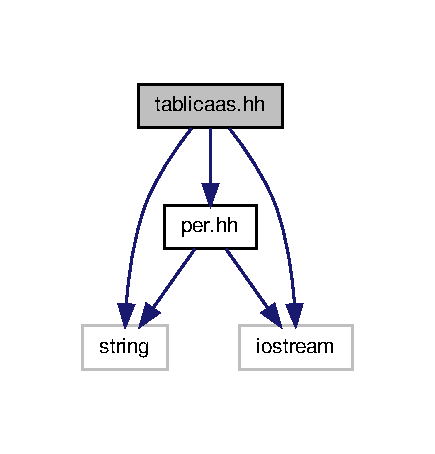
\includegraphics[width=216pt]{tablicaas_8hh__incl}
\end{center}
\end{figure}
Ten wykres pokazuje, które pliki bezpośrednio lub pośrednio załączają ten plik\-:\nopagebreak
\begin{figure}[H]
\begin{center}
\leavevmode
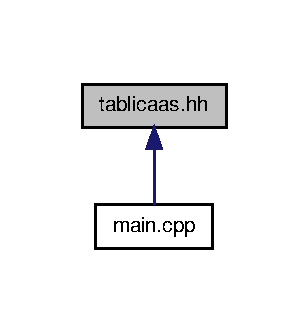
\includegraphics[width=216pt]{tablicaas_8hh__dep__incl}
\end{center}
\end{figure}
\subsection*{Komponenty}
\begin{DoxyCompactItemize}
\item 
class \hyperlink{class_tablicaas}{Tablicaas$<$ K, W $>$}
\begin{DoxyCompactList}\small\item\em Modeluje pojęcie \hyperlink{class_tablicaas}{Tablicaas}. Klasa modeluje pojęcie Tablica asocjacyjna . Jej atrybutem są pola zawierające klucz i wartość. \end{DoxyCompactList}\end{DoxyCompactItemize}
\subsection*{Definicje}
\begin{DoxyCompactItemize}
\item 
\#define \hyperlink{tablicaas_8hh_aa50aa866c5823769bb02e986d29a0589}{R\-O\-Z\-M\-I\-A\-R}~1000000
\end{DoxyCompactItemize}


\subsection{Opis szczegółowy}
Plik zawiera definicję szablonu klasy Tablicaas.\-Jest to klasa główna , która wykorzystuje klasę per. 

Definicja w pliku \hyperlink{tablicaas_8hh_source}{tablicaas.\-hh}.



\subsection{Dokumentacja definicji}
\hypertarget{tablicaas_8hh_aa50aa866c5823769bb02e986d29a0589}{\index{tablicaas.\-hh@{tablicaas.\-hh}!R\-O\-Z\-M\-I\-A\-R@{R\-O\-Z\-M\-I\-A\-R}}
\index{R\-O\-Z\-M\-I\-A\-R@{R\-O\-Z\-M\-I\-A\-R}!tablicaas.hh@{tablicaas.\-hh}}
\subsubsection[{R\-O\-Z\-M\-I\-A\-R}]{\setlength{\rightskip}{0pt plus 5cm}\#define R\-O\-Z\-M\-I\-A\-R~1000000}}\label{tablicaas_8hh_aa50aa866c5823769bb02e986d29a0589}


Definicja w linii 10 pliku tablicaas.\-hh.


\addcontentsline{toc}{part}{Indeks}
\printindex
\end{document}
